% Recta real con números notables (TikZ) — Eric Lucero González — https://ericlucero.dev
% Licencia CC BY-NC-SA 4.0. Compilar con pdfLaTeX.
\documentclass[tikz, border=5mm]{standalone}
\usepackage{amsmath}

% Colores (cámbialos a tu gusto)
\definecolor{purpleA}{HTML}{6A1B9A}
\definecolor{purpleB}{HTML}{9C27B0}
\definecolor{purpleC}{HTML}{BA68C8}

% Valores aproximados para colocar cada número
\def\e{2.718}
\def\minusSq{-1.414}
\def\halfA{0.5}
\def\halfB{-2.0943}
\def\halfC{2.665144}

\begin{document}
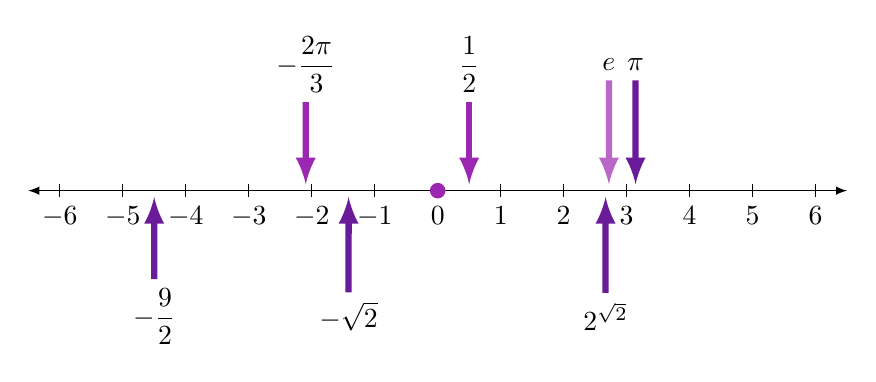
\begin{tikzpicture}[scale=0.8]
  \coordinate (piDown) at (3.14159,0.1);
  \coordinate (aDown) at (\e,0.1);
  \coordinate (bDown) at (\minusSq,-0.1);
  \coordinate (cDown) at (\halfA,0.1);
  \coordinate (dDown) at (\halfB,0.1);
  \coordinate (eDown) at (\halfC,-0.1);
  \coordinate (fDown) at (-4.5,-0.1);
  \node (piUp) at (3.14159,2) {$\pi$};
  \node (aUp) at (\e,2) {$e$};
  \node (bUp) at (\minusSq,-2) {$-\sqrt{2}$};
  \node (cUp) at (\halfA,2) {$\dfrac{1}{2}$};
  \node (dUp) at (\halfB,2) {$-\dfrac{2\pi}{3}$};
  \node (eUp) at (\halfC,-2) {$2^{\sqrt{2}}$};
  \node (fUp) at (-4.5,-2) {$-\dfrac{9}{2}$};
  \draw[latex-latex] (-6.5,0) -- (6.5,0);
  \foreach \x in {-6,...,6}
  \draw[shift={(\x,0)}] (0pt,3pt) -- (0pt,-3pt) node[below] {$\x$};
  \draw[purpleB, thick, fill=purpleB] (0,0) circle (3pt);
  \draw[-latex, line width=0.8mm, purpleA] (piUp) -- (piDown);
  \draw[-latex, line width=0.8mm, purpleC] (aUp) -- (aDown);
  \draw[-latex, line width=0.8mm, purpleA] (bUp) -- (bDown);
  \draw[-latex, line width=0.8mm, purpleB] (cUp) -- (cDown);
  \draw[-latex, line width=0.8mm, purpleB] (dUp) -- (dDown);
  \draw[-latex, line width=0.8mm, purpleA] (eUp) -- (eDown);
  \draw[-latex, line width=0.8mm, purpleA] (fUp) -- (fDown);
\end{tikzpicture}
\end{document}
